\documentclass[twocolumn,english]{article}
\usepackage[latin9]{inputenc}
\usepackage[landscape]{geometry}
\geometry{verbose,tmargin=0.5in,bmargin=0.75in,lmargin=0.5in,rmargin=0.5in}
\setlength{\parskip}{0bp}
\setlength{\parindent}{0pt}
\usepackage{float}
\usepackage{booktabs}
\usepackage{amsmath}
\usepackage{graphicx}

\makeatletter

\providecommand{\tabularnewline}{\\}




\usepackage{array}
\usepackage{multirow}
\usepackage{amsbsy}




\providecommand{\tabularnewline}{\\}

\setlength{\columnsep}{0.25in}
\usepackage{xcolor}
\usepackage{textcomp}
\usepackage{listings}
\lstset{
  tabsize=2,
  basicstyle=\small\ttfamily,
}



\usepackage{babel}
\usepackage{listings}
\renewcommand{\lstlistingname}{Listing}

\makeatother

\usepackage{babel}
\begin{document}

\title{Reference Sheet for C221 Compilers}

\date{Autumn 2017}
\maketitle

\section{Lexical Analysis}

Transforms a stream of characters into tokens.

\subsection{Tokens}

\paragraph{Identifier Tokens}
\begin{itemize}
\item \emph{Keyword identifiers}, e.g. \texttt{while} - generally have their
own token.
\item \emph{Non-keyword identifiers} - have a general identifier token e.g.
\texttt{IDENT(\char`\"{}year\char`\"{})}.
\end{itemize}
Use a fast lookup function to determine if a scanned identifier is
a keyword (e.g. perfect hash).

\paragraph{Literal Tokens}
\begin{itemize}
\item \emph{Unsigned integers} - represented by a token for integers, plus
an integer.
\item \emph{Unsigned reals}, \emph{strings} represented similarly.
\end{itemize}

\paragraph{Other Tokens}
\begin{itemize}
\item \emph{1 or 2-char symbols}, e.g. +, \textless{}= usually represented
by their own token.
\item \emph{Whitespace} and \emph{comments} usually not represented in token
stream.
\item \emph{Macros} usually removed before lexical analysis.
\end{itemize}

\subsection{Regular Expressions}

\begin{table}[H]
\centering{}%
\begin{tabular}{cc}
\toprule 
 & \textbf{\footnotesize{}Matches}\tabularnewline
\midrule
\texttt{a} & {\footnotesize{}Symbol}\tabularnewline
$\epsilon$ & {\footnotesize{}Empty string}\tabularnewline
\texttt{R1 R2} & \texttt{\footnotesize{}R1}{\footnotesize{} followed by }\texttt{\footnotesize{}R2}\tabularnewline
\texttt{R1\textbar{}R2} & \texttt{\footnotesize{}R1}{\footnotesize{} or }\texttt{\footnotesize{}R2}\tabularnewline
\texttt{R{*}} & {\footnotesize{}0 or more occurrence of }\texttt{\footnotesize{}R}\tabularnewline
\texttt{(R)} & \texttt{\footnotesize{}R}\tabularnewline
\texttt{\textbackslash{}a} & {\footnotesize{}Escaped symbol}\tabularnewline
\midrule
\texttt{R?} & {\footnotesize{}0 or 1 occurrence of }\texttt{\footnotesize{}R}\tabularnewline
\texttt{R+} & {\footnotesize{}1 or more occurrence of }\texttt{\footnotesize{}R}\tabularnewline
\texttt{{[}a-zA-Z{]}} & {\footnotesize{}Any character from given set}\tabularnewline
\texttt{{[}\textasciicircum{}a-zA-Z{]}} & {\footnotesize{}Any character except from given set}\tabularnewline
\texttt{.} & {\footnotesize{}Any character except newline}\tabularnewline
\bottomrule
\end{tabular}
\end{table}


\subsection{Rules}

\paragraph{Regular Expression Rules}

\emph{Rules} (\emph{productions}) of the form $\alpha\rightarrow\texttt{X}$
where $\alpha$ is a \emph{non-terminal} (name of rule) and \texttt{X}
is a regular expression constructed from both non-terminals and terminals
(input chars).

\emph{Note} that non-terminals must be defined before use, and recursion
is not allowed.

E.g.
\begin{itemize}
\item $\texttt{Digit}\rightarrow\texttt{[0-9]}$
\item $\texttt{Int}\rightarrow\texttt{Digit+}$
\end{itemize}

\paragraph{Disambiguation Rules}
\begin{itemize}
\item Use longest matching character sequence.
\item Assume regular expressions have textual precedence.
\end{itemize}

\paragraph{Implementation}

Either hand-crafted, or use lexical analyser generator (e.g. Flex).

\begin{figure}[H]
\begin{centering}
\emph{Lexical analyser generator}:
\par\end{centering}
\centering{}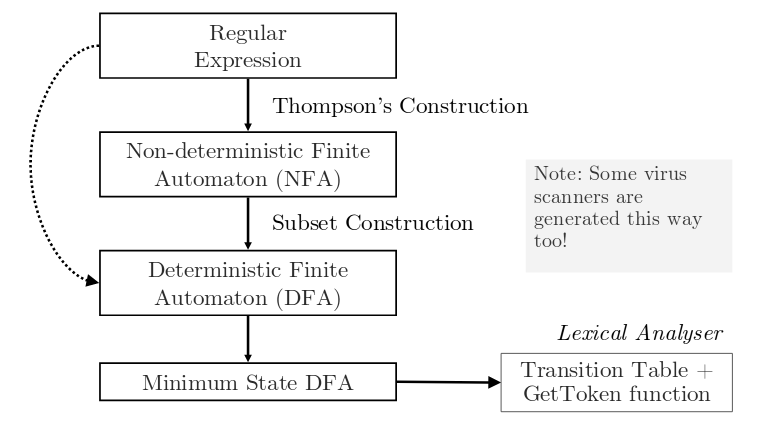
\includegraphics[width=0.75\linewidth]{img/lex}
\end{figure}


\subsection{Finite Automata}
\begin{itemize}
\item \emph{States} of matching process (circles).
\item \emph{Transitions} between those states (arrows).
\item Matched input \emph{symbols} (labels on transitions).
\item \emph{Accepting states} of matching process (double circle).
\item \emph{Start state} (unlabelled incoming arrow).
\end{itemize}

\paragraph{Deterministic Finite Automata}

No two transitions leaving a state have the same symbol.

\paragraph{Non-deterministic Finite Automata}

Allow a choice of transitions out of a state

\paragraph{Thompson's Construction}

Use $\epsilon$ transitions to glue together automata for each part
of a regex:

\begin{figure}[H]
\begin{centering}
\texttt{r1 r2}
\par\end{centering}
\centering{}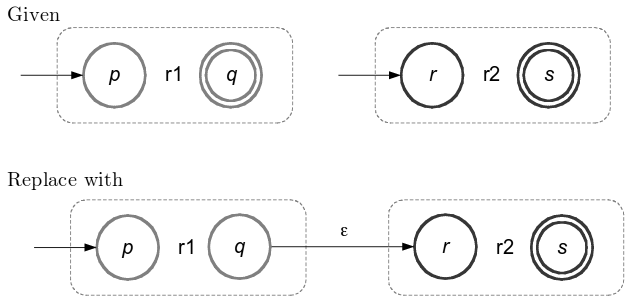
\includegraphics[width=0.5\linewidth]{img/concat}
\end{figure}

\begin{figure}[H]
\begin{centering}
\texttt{r1\textbar{}r2}
\par\end{centering}
\centering{}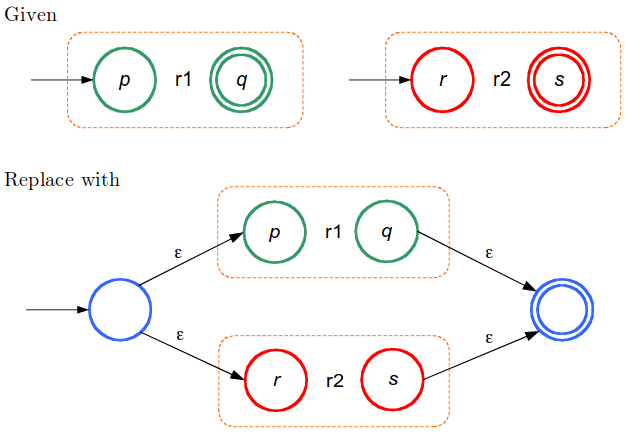
\includegraphics[width=0.5\linewidth]{img/alternate}
\end{figure}

\begin{figure}[H]
\begin{centering}
\texttt{r1{*}}
\par\end{centering}
\centering{}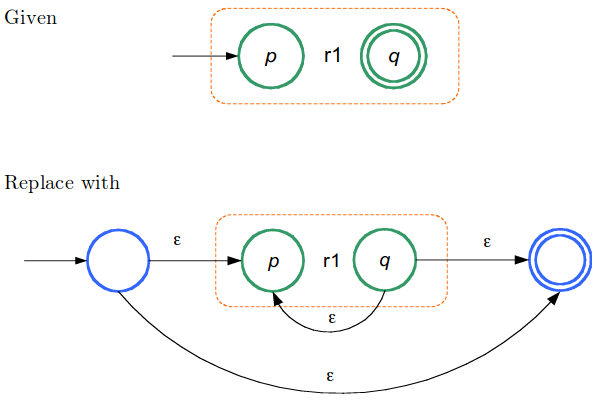
\includegraphics[width=0.5\linewidth]{img/repeat}
\end{figure}


\paragraph{Subset Construction}
\begin{itemize}
\item DFAs are much faster than NFAs (linear on size of input string), 
\item but require more memory (potentially $2^{n}$ states for an $n$-state
NFA).
\end{itemize}
\emph{Algorithm}:
\begin{enumerate}
\item DFA start state = $\epsilon$ closure of NFA start state.
\item For each new subset state $S$ of the DFA:
\begin{enumerate}
\item For each unique symbol \texttt{a} leading out from any state of $S$:
\begin{enumerate}
\item Add a transition \texttt{a} from S to S' where S' = $\epsilon$ closure
of states reached by \texttt{a}
\end{enumerate}
\end{enumerate}
\end{enumerate}

\paragraph{Generating a Lexical Analyser}

Encode DFA as a 2D table of states (row per state, col per char).

\section{Parsing}

Transforms a stream of tokens to an AST tree based on context free
grammar of the language.

\subsection{LR (Bottom-Up / Shift-Reduce) Parsing}
\begin{itemize}
\item Can be implemented in $O(n)$ time.
\item Several methods for generating LR parsing tables. States consist of
LR(k) items of the grammar, vary in number of states and size of lookahead
sets.
\end{itemize}

\subsubsection{LR(0) Parsing}

Don't use the current token in order to perform a reduce. E.g the
rule $\texttt{X}\rightarrow\texttt{ABC}$ has 4 LR(0) items, where
$\bullet$ indicates how much of the rule we have seen:
\begin{enumerate}
\item $\texttt{X}\rightarrow\texttt{\ensuremath{\bullet}ABC}$ 
\item $\texttt{X}\rightarrow\texttt{A\ensuremath{\bullet}BC}$ 
\item $\texttt{X}\rightarrow\texttt{AB\ensuremath{\bullet}C}$ 
\item $\texttt{X}\rightarrow\texttt{ABC\ensuremath{\bullet}}$ 
\end{enumerate}

\paragraph{LR(0) to Finite Automata}

Given $\texttt{X}\rightarrow\texttt{A\ensuremath{\bullet}BC}$, we
add the transition:

\begin{figure}[H]
\centering{}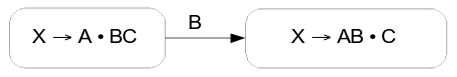
\includegraphics[width=0.4\linewidth]{img/lr0tonfa}
\end{figure}

Suppose \texttt{B} is a non-terminal, then for all $\texttt{B}\rightarrow\texttt{\ensuremath{\bullet}D}$,
we add $\epsilon$ transitions of the form:

\begin{figure}[H]
\centering{}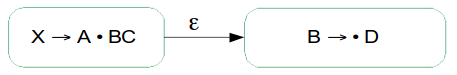
\includegraphics[width=0.4\linewidth]{img/lr0tonfa-nonterminal}
\end{figure}

We then construct a DFA using subset construction.

\paragraph{Finite Automata to Parsing Table}
\begin{enumerate}
\item For each terminal transition $\texttt{X}\xrightarrow{\texttt{T}}\texttt{Y}$,
add $\texttt{P}[\texttt{X},\texttt{T}]=s\texttt{Y}$ (\textbf{shift}
\texttt{Y}).
\item For each non-terminal transition $\texttt{X}\xrightarrow{\texttt{N}}\texttt{Y}$,
add $\texttt{P}[\texttt{X},\texttt{N}]=g\texttt{Y}$ (\textbf{goto}
\texttt{Y}).
\item For each state \texttt{X} containing the item $\texttt{R'}\rightarrow\dots\bullet$,
add $\texttt{P}[\texttt{X},\texttt{\$}]=a$ (\textbf{accept}).
\item For each state \texttt{X} containing the item $\texttt{R}\rightarrow\dots\bullet$,
add $\texttt{P}[\texttt{X},\texttt{T}]=rN$ (\textbf{reduce}), for
every terminal \texttt{T} where $N$ is $R$'s rule number.
\end{enumerate}

\paragraph{Model of an LR Parser}

Modelled by pushdown automata:
\begin{itemize}
\item \emph{Shift} pushes state onto stack and advances token.
\item \emph{Reduce}:
\begin{itemize}
\item removes $L$ tokens from the stack ($L$ is the length of the RHS
of the rule), 
\item pushes the state of the \emph{goto} for the LHS of the rule according
to the state now on the top of the stack,
\item and generates an AST node for the rule.
\end{itemize}
\end{itemize}

\subsubsection{Other LR Parsing Methods}
\begin{itemize}
\item \emph{FIRST set} for a sequence of non-terminals and terminals $\alpha$
is the set of all tokens that could start a derivation of $\alpha$,
including $\epsilon$ if $\alpha$ can derive $\epsilon$.
\begin{itemize}
\item A non-terminal \texttt{A} is \emph{nullable} if $A\implies^{*}\epsilon$.
\end{itemize}
\item \emph{FOLLOW set} for a non-terminal \texttt{A} is the set of all
tokens that could immediately follow \texttt{A}, including \texttt{\$}
if \texttt{A} can end the input.
\end{itemize}

\paragraph{Different LR Parsers}
\begin{itemize}
\item LR(0): A reduce item $\texttt{X}\rightarrow\texttt{A\ensuremath{\bullet}}$
always causes a reduction.
\item SLR(1): A reduce item $\texttt{X}\rightarrow\texttt{A\ensuremath{\bullet}}$
causes a reduction only if the current token is in FOLLOW(\texttt{X}).
\item LR(1): A reduce item $\texttt{X}\rightarrow\texttt{A\ensuremath{\bullet}},\texttt{t}$
causes a reduction only if the current token is \texttt{t}.
\item LALR(1): Combines LR(1) states that differ in the look-ahead token
only. This can cause spurious reductions before an error is detected.
\end{itemize}

\subsubsection{Ambiguities}

Grammars which can derive more than 1 parse tree for some input cannot
be LR($k$) for any $k$.

\paragraph{Shift-Reduce Conflicts}

Consider the grammar:

\begin{alignat*}{2}
\texttt{S} & \rightarrow & if\texttt{ E }then\texttt{ S }else\texttt{ S}\\
\texttt{S} & \rightarrow & if\texttt{ E }then\texttt{ S}\\
\texttt{S} & \rightarrow & id\\
\texttt{E} & \rightarrow & 0\mid1
\end{alignat*}

and the statement:
\[
if\texttt{ a }then\texttt{ }if\texttt{ b }then\texttt{ c }else\texttt{ d}
\]

\begin{itemize}
\item If we shift first, we get: $if\texttt{ a }then\texttt{ }\boxed{if\texttt{ b }then\texttt{ c }else\texttt{ d}}$.
\item If we reduce first, we get: $if\texttt{ a }then\texttt{ }\boxed{if\texttt{ b }then\texttt{ c}}\texttt{ }else\texttt{ d}$.
\end{itemize}
\emph{Solution}: rewrite the grammar:
\begin{align*}
\texttt{S} & \rightarrow & \texttt{MatchedS}\\
\texttt{MatchedS} & \rightarrow & if\texttt{ E }then\texttt{ MatchedS }else\texttt{ MatchedS}\\
\texttt{MatchedS} & \rightarrow & id
\end{align*}
\begin{align*}
\texttt{S} & \rightarrow & \texttt{UnmatchedS}\\
\texttt{UnmatchedS} & \rightarrow & if\texttt{ E }then\texttt{ S}\\
\texttt{UnmatchedS} & \rightarrow & if\texttt{ E }then\texttt{ MatchedS }else\texttt{ UnmatchedS}
\end{align*}

We now force $else$-parts to become matched as soon as possible.

\paragraph{Reduce-Reduce Conflicts}

Consider the grammar:
\[
\texttt{Expr}\rightarrow\texttt{Expr `+' Expr}\mid\texttt{Expr `*' Expr}\mid\texttt{`(' Expr `)'}\mid int
\]

This is ambiguous because it doesn't define the associativity or precedence
of \texttt{+} and \texttt{{*}}.

\emph{Solution}: rewrite the grammar:
\begin{align*}
\texttt{Expr} & \rightarrow & \texttt{Expr `+' Term}\mid\texttt{Term}\\
\texttt{Term} & \rightarrow & \texttt{Term `*' Factor}\mid\texttt{Factor}\\
\texttt{Factor} & \rightarrow & \texttt{`(' Expr `)'}\mid int
\end{align*}


\paragraph{Parse Trees}

Build leaf nodes for each input token (\emph{shift}) and non-leaf
nodes for each rule (\emph{reduce}).

\paragraph{Abstract Syntax Trees}

Remove unnecessary information from the parse tree - can be constructed
by a separate parse or by attaching AST construction code directly
to grammar rules.
\end{document}
